\begin{figure}[t]
    \centering
    \vspace{-3mm}
    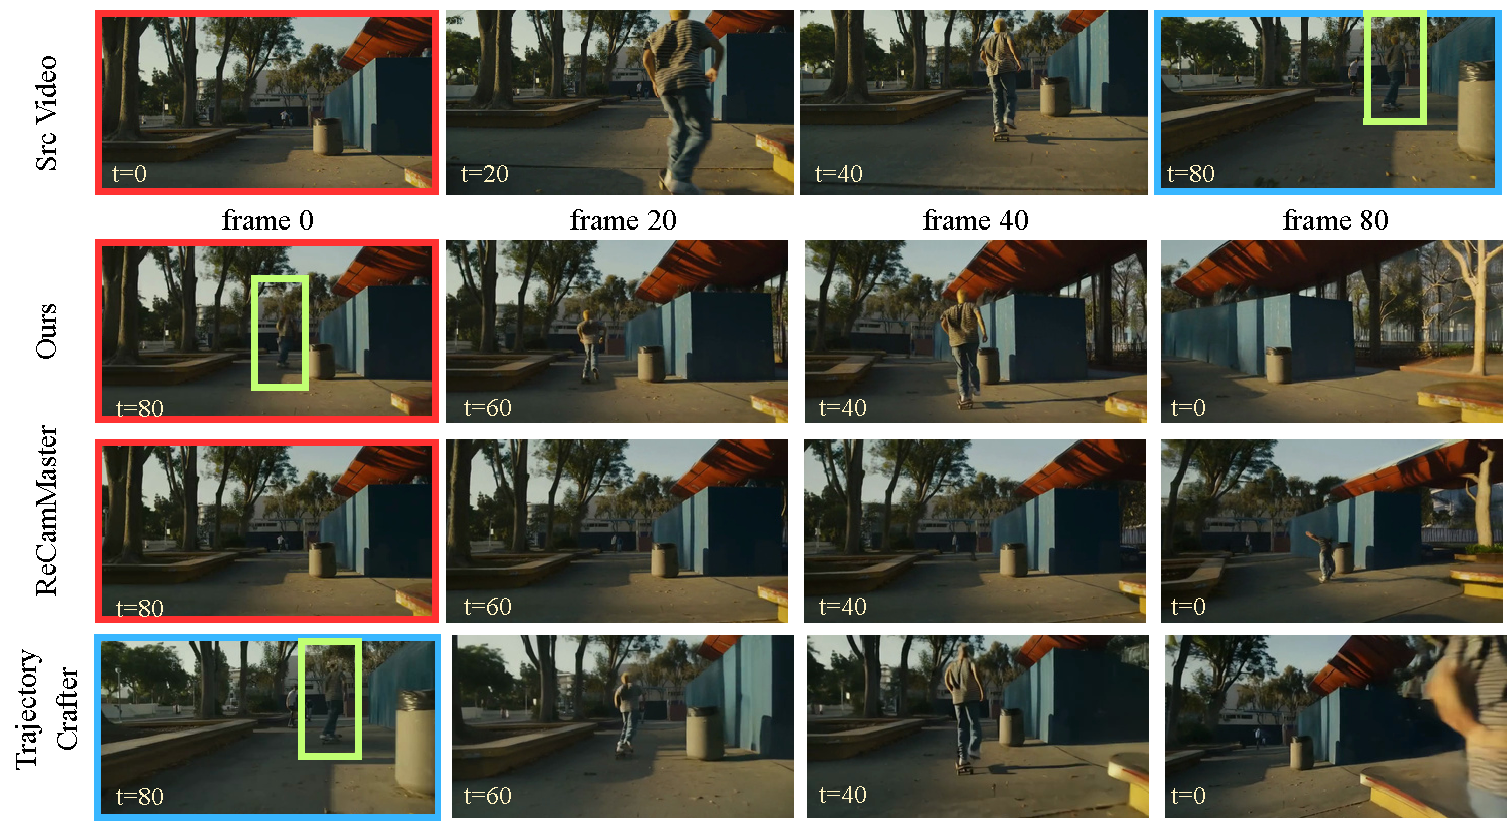
\includegraphics[width=\linewidth,trim={0 0 0 0},clip]{figures/src_files/Comparison_2.pdf}
    \caption{
    \textbf{Qualitative comparison of disentangled camera-time control.}  In this example, we apply reverse playback (time) and a pan-right camera motion starting from the first-frame pose to a source video (top), whose original camera motion is dolly-in (red to blue). SpaceTimePilot, by explicitly disentangling space and time, achieves correct camera control (red boxes) together with accurate temporal control (green boxes). For TrajectoryCrafter, it  first reverses the frames and then apply their method for viewpoint control, resulting in incorrect  camera motion. ReCamMaster (with joint-dataset training) is unable to perform temporal control, leading to failure cases.}
    \label{fig:disentangle}
\end{figure}



